
\section{Specific Requirements}\label{sec:specific-requirements}
    \subsection{External Interface Requirements}\label{sec:external-interface-requirements}
        \subsubsection{User Interfaces}\label{sec:user-interfaces}
            % \emph{Describe the logical characteristics of each interface between the software product and the users. This may include sample screen images, any GUI standards or product family style guides that are to be followed, screen layout constraints, standard buttons and functions (e.g., Cancel) that will appear on every screen, error message display standards, and so on. Define the software components for which a user interface is needed.\gnl The least you can do for this section is to describe in words the different User Interfaces and the different screens that will be available to the user. Optional: You may also provide an initial Graphical User Interface design (does not have to be final).}
            There should be a simple homepage that provides a brief description of the product and allows users to log in. Upon logging in, they will be presented with a dashboard pertaining to their user group(s). From the dashboard, they can access allowed functionality and get a summary of recent or upcoming activity. Inter-user communication functionality will be accessed via a separate view with a list of current conversations and history of previous messages. From every screen, users can navigate back to their dashboard, the \projectName\ homepage, or quickly access other functionality-specific pages.
            \par The style should be minimal and follow \gls{material-design} guidelines. Text information should be moderately dense but easily readable, and images or canvases used to present meaningful information. Users can select between a dark or light theme.
        \subsubsection{Hardware Interfaces}\label{sec:hardware-interfaces}
            % \emph{Describe the logical and physical characteristics of each interface between the software product and the hardware components of the system. This may include the supported device types, the nature of the data and control interactions between the software and the hardware. You are not required to specify what protocols you will be using to communicate with the hardware, but it will be usually included in this part as well.\gnl Please provide a short description of the different hardware interfaces. If you will be using some special libraries to communicate with your software mention them here. In case you have more than one hardware interface divide this section into subsections.}
            The user-facing product will be usable from both desktop and mobile web clients. We will be using \gls{vue} as our front-end framework while following \gls{responsive} principles. The system will use common web APIs for requesting file uploads and interactions with the user's \gls{os}. The views and functionality will be nearly identical between hardware interfaces, but the layout will change according to screen size and hardware type.
            \par The backend is designed to run containerized\dots % TODO
        \subsubsection{Software Interfaces}\label{sec:software-interfaces}
            \emph{Describe the connections between this product and other specific software components (name and version), including databases, operating systems (Windows? Linux? Etc\dots), tools, libraries, and integrated commercial components. Identify the data items or messages coming into the system and going out and describe the purpose of each. Describe the services needed and the nature of communications. Identify data that will be shared across software components. If the data sharing mechanism must be implemented in a specific way (for example, use of a global data area in a multitasking operating system), specify this as an implementation constraint.\gnl The previous part illustrates some of the information you would usually include in this part of the SRS document. To make things simpler, you are only required to describe the specific interface with the operating system.}
        \subsubsection{Communications Interfaces}\label{sec:communications-interfaces}
            \emph{Describe the requirements associated with any communications functions required by this product, including e-mail, web browser, network server communications protocols, electronic forms, and so on. Define any pertinent message formatting. Identify any communication standards that will be used, such as FTP or HTTP. Specify any communication security or encryption issues, data transfer rates, and synchronization mechanisms.\gnl Do not go into too much detail, but provide 1-2 paragraphs were you will outline the major communication standards. For example, if you decide to use encryption there is no need to specify the exact encryption standards, but rather, specify the fact that the data will be encrypted and name what standards you consider using.}
    \subsection{Functional Requirements}\label{sec:functional-requirements}
        % \emph{Functional requirements capture the intended behavior of the system. This behavior may be expressed as services, tasks or functions the system is required to perform. This section is the direct continuation of section 2.2 where you have specified the general functional requirements. Here, you should list in detail the different product functions with specific explanations regarding every function.\gnl Break the functional requirements to several functional areas and divide this section into subsections accordingly. Provide a detailed list of all product operations related to these functional areas.}
        \subsubsection{Administrative}\label{sec:administrative-functions}
            \begin{itemize}
                \item \textbf{Manage a user's groups and relationships to other users}. Since a user can be in multiple user groups simultaneously, as in the case of a school owner still giving their own lessons, there will be functionality to add/remove their own user groups and set up an association with another user. Certain functionalities will be disabled according to the permissions described below.
                \item \textbf{Manage permissions of user groups and individual users}. Varying permission levels are needed to suit a wide range of users. Instructors and schools will be able to set up policies for what their lower-permission users have access to, such as adding students or withdrawing from lessons with no notice.
            \end{itemize}
        \subsubsection{File Management}\label{sec:file-management-functions}
            \begin{itemize}                
                % \item \textbf{Create and share file templates}. 
                \item \textbf{Share files with specific read/write permissions to other users}. File-sharing is important for users to share documents such as \glspl{lesson plan} and \glspl{practice-resource} with each other. Instructors could collaborate together to improve a \gls{practice-resource} or give a substitute instructor their students' \glspl{lesson plan}. This is also how instructors will share \glspl{lesson plan} with their students.
                \item \textbf{View upcoming scheduled lessons}. Any given user's dashboard will display information on the nearest upcoming lessons. Students will see their next lesson's date and details, instructors will see a list of upcoming lessons for the next day/week, and schools will see a list of their teachers' lessons for easy navigation.
                \item \textbf{Automated creation and backups of weekly \glspl{lesson plan}}. To partially automate the management of students, the product will create copies of the previous \gls{lesson plan} and update the date within the document to match the next lesson's date. \Glspl{lesson plan} will also be organized and archived to allow for viewing a student's progress.
            \end{itemize}
        \subsubsection{Communications}\label{sec:communications-functions}
            \begin{itemize}
                \item \textbf{Message other users with varying priority levels}. Users with the correct permissions can communicate through the product. The varying priority levels are for flexibility of sending messages of different importance. This will be implemented internally, with permissions to control the priority levels. 
            \end{itemize}
        \subsubsection{3rd-Party Integration}\label{sec:3rd-party-integration-functions}
            \begin{itemize}                
                \item \textbf{Scheduling with Google Calendar}. The product will rely on Google Calendar rather than an internal calendar implementation. Google Calendar will be the backend for managing and storing schedule data. Users will not interact directly with Google Calendar, but instead with a simpler interface that abstracts away the details of creating recurring events for lessons.
            \end{itemize}
    \subsection{Behavior Requirements}\label{sec:behavior-requirements}
        \subsubsection{Use Case View}\label{sec:use-case-view}
            % \emph{A use case defines a goal-oriented set of interactions between external actors and the system under consideration.\gnl Provide a use case diagram which shows the entire system and all possible actors. Do not include detailed use case descriptions (these will be needed when you will be working on the Test Plan), but make sure to include a short description of what every use-case is, who are the actors in your diagram.}
            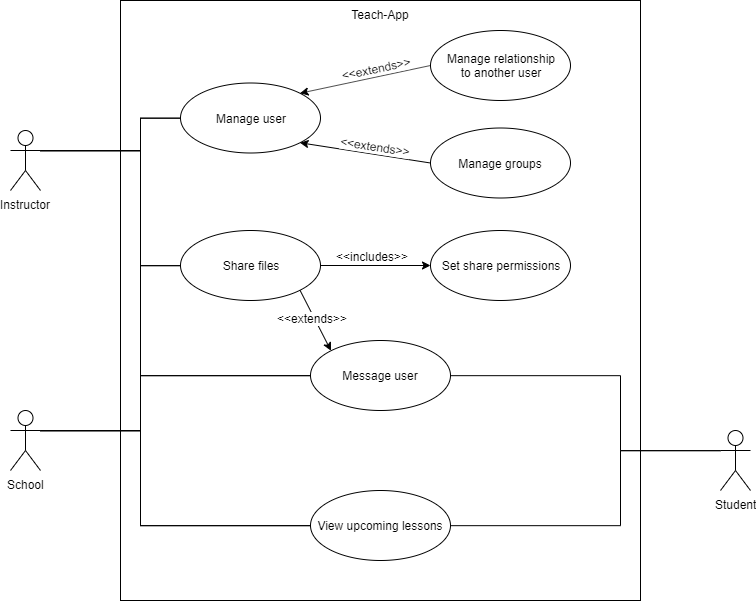
\includegraphics[width=\textwidth]{images/Use-Case-Diagram.png}
